\subsection{Hiểu Dữ Liệu (Data Understanding)}


\subsubsection{Nguồn dữ liệu và mô tả bài toán}
Bộ dữ liệu được sử dụng là dữ liệu hành tinh ngoài Hệ Mặt Trời từ NASA Exoplanet Archive.
File \texttt{planet.csv} hiện có 4636 dòng và 320 cột
\begin{center}
    \texttt{part2/data/planet.csv}.
\end{center}

Pipeline đọc trực tiếp file full-column này, sau đó thực hiện bước \emph{schema filter} ngay ở đầu
\texttt{DataPipeline}: từ 320 cột chỉ giữ lại 16 cột ứng viên có ý nghĩa vật lý cho mô hình (giải thích chi tiết ở phần sau)
(\texttt{pl\_orbper}, \texttt{pl\_orbsmax}, \texttt{pl\_orbeccen}, \texttt{pl\_trandur},
\texttt{pl\_trandep}, \texttt{pl\_imppar}, \texttt{pl\_eqt}, \texttt{pl\_insol},
\texttt{pl\_bmasse}, \texttt{st\_teff}, \texttt{st\_rad}, \texttt{st\_mass},
\texttt{st\_met}, \texttt{st\_logg}, \texttt{sy\_dist}, \texttt{pl\_rade}) và loại 304 cột metadata/nhiễu còn lại.

Sau bước schema filter, pipeline áp dụng ràng buộc miền để tập trung vào nhóm hành
tinh đá/Super-Earth:
\begin{equation}
    \texttt{pl\_rade} \le 1.6,\qquad \texttt{pl\_bmasse} \le 10,
\end{equation}
số mẫu còn lại dùng cho EDA và mô hình hóa là 1084 dòng.

Lý do của bước lọc này đến từ cơ chế vật lý của dữ liệu. Động lực vật lý
(\emph{physical mechanics}) cấu trúc nên một hành tinh khí khổng lồ
(\emph{Gas Giant}) khác đáng kể so với một hành tinh đá
(\emph{Terrestrial}) hoặc Super-Earth. Nếu giữ nguyên toàn bộ tập dữ liệu, mặt phẳng hồi quy sẽ
phải đồng thời mô tả nhiều chế độ vật lý khác nhau, dễ bị nhiễu bởi hiện tượng phương sai không
đồng nhất (\emph{heteroskedasticity}) do chênh lệch quy mô quá lớn giữa các nhóm hành tinh.
Vì vậy, nhóm quyết định thực hiện trên nhóm hành tinh đá và Super-Earth, nhằm tối ưu hóa khả năng nội suy
cục bộ của mô hình bằng cách chỉ giữ nhóm hành tinh đá và
Super-Earth theo ngưỡng phân rã Fulton (\emph{Fulton Gap}): bán kính không vượt quá
$1.6\,R_\oplus$ và khối lượng không vượt quá $10\,M_\oplus$. Thao tác này được thực hiện trong
pipeline ngay sau schema filter và trước train/test split, MICE, VIF cũng như chuẩn hóa. Nhờ đó,
bộ nội suy MICE và các tham số mean/std chỉ học đặc trưng phân phối của riêng nhóm hành tinh đá và
Super-Earth.

\begin{table}[H]
\centering
\caption{Quy mô dữ liệu qua các bước chính}
\label{tab:part2_data_size}
\begin{tabular}{@{}lrrp{0.38\textwidth}@{}}
\hline
\textbf{Giai đoạn} & \textbf{Số dòng} & \textbf{Số cột} & \textbf{Ghi chú} \\
\hline
\texttt{planet.csv} & 4636 & 320 & Dữ liệu chuẩn ban đầu của Phần 2 \\
Sau schema filter & 4636 & 16 & Pipeline giữ 16 cột ứng viên vật lý và loại 304 cột metadata/sai số/tham chiếu. \\
Sau domain restriction & 1084 & 16 & Giữ các mẫu có \texttt{pl\_rade}$\le1.6$ và \texttt{pl\_bmasse}$\le10$. \\
Train sau tiền xử lý & 867 & 11 & Dùng để fit preprocessing và mô hình. \\
Test sau tiền xử lý & 217 & 11 & Chỉ dùng để đánh giá cuối cùng. \\
\hline
\end{tabular}
\end{table}

\subsubsection{Các biến trong dữ liệu}

\begin{table}[H]
\centering
\caption{Nhóm biến được giữ sau schema filter trong pipeline}
\label{tab:part2_variables}
\begin{tabular}{@{}p{0.22\textwidth}p{0.35\textwidth}p{0.34\textwidth}@{}}
\hline
\textbf{Nhóm biến} & \textbf{Tên biến} & \textbf{Ý nghĩa} \\
\hline
Quỹ đạo & \texttt{pl\_orbper}, \texttt{pl\_orbsmax}, \texttt{pl\_orbeccen}
& Chu kỳ quỹ đạo, bán trục lớn, độ lệch tâm. \\
Transit & \texttt{pl\_trandur}, \texttt{pl\_trandep}, \texttt{pl\_imppar}
& Thời lượng transit, độ sâu transit và impact parameter. \\
Năng lượng & \texttt{pl\_eqt}, \texttt{pl\_insol}
& Nhiệt độ cân bằng và thông lượng bức xạ nhận từ sao chủ. \\
Hành tinh & \texttt{pl\_bmasse}, \texttt{pl\_rade}
& Khối lượng và bán kính hành tinh. \\
Sao chủ & \texttt{st\_teff}, \texttt{st\_rad}, \texttt{st\_mass}, \texttt{st\_met}, \texttt{st\_logg}
& Nhiệt độ hiệu dụng, bán kính, khối lượng, kim loại tính và log-g của sao chủ. \\
Hệ sao & \texttt{sy\_dist}
& Khoảng cách từ Trái Đất đến hệ sao. \\
\hline
\end{tabular}
\end{table}

\begin{table}[H]
\centering
\caption{Một vài dòng dữ liệu mẫu sau schema filter và trước domain restriction}
\label{tab:part2_sample_data}
\resizebox{\textwidth}{!}{%
\begin{tabular}{@{}rrrrrrrr@{}}
\hline
\textbf{\texttt{pl\_orbper}} & \textbf{\texttt{pl\_orbsmax}} & \textbf{\texttt{pl\_trandur}} &
\textbf{\texttt{pl\_trandep}} & \textbf{\texttt{pl\_bmasse}} & \textbf{\texttt{st\_teff}} &
\textbf{\texttt{sy\_dist}} & \textbf{\texttt{pl\_rade}} \\
\hline
1.0039 & 0.0175 & 1.4562 & 0.04911 & 3.570 & 4971 & 820.905 & 1.710 \\
8.1724 & 0.0779 & 3.9020 & 0.08643 & 11.000 & 5705 & 1061.770 & 3.323 \\
6.2839 & 0.0687 & 4.1240 & 0.00357 & 0.437 & 6022 & 493.175 & 0.800 \\
3.1739 & 0.0464 & 3.5066 & 0.03030 & 10.100 & 6747 & 1318.050 & 3.150 \\
56.3585 & 0.2698 & 6.9270 & 0.25596 & 18.700 & 5446 & 962.888 & 4.541 \\
\hline
\end{tabular}}
\end{table}

Bảng mẫu cho thấy lý do cần ràng buộc miền trước khi mô hình hóa: một số hành tinh có bán kính và
khối lượng vượt xa nhóm hành tinh đá/Super-Earth. Nếu trộn chung các nhóm vật lý khác nhau, mô
hình tuyến tính dễ học một quan hệ trung bình kém ổn định.

\subsubsection{Khám phá dữ liệu ban đầu}

Các thống kê mô tả trên 1084 mẫu sau domain restriction được tóm tắt trong
Bảng~\ref{tab:part2_describe}. Dữ liệu có thang đo rất khác nhau: \texttt{pl\_orbper} dao động từ
0.1769 đến 199.6688 ngày, \texttt{pl\_insol} từ 0.144 đến 8385.9, còn \texttt{sy\_dist} từ
6.8693 đến 2712.58. Đây là tín hiệu rõ rằng cần biến đổi thang đo trước khi hồi quy.

\begin{table}[H]
\centering
\caption{Thống kê mô tả của một số biến số sau domain restriction}
\label{tab:part2_describe}
\resizebox{\textwidth}{!}{%
\begin{tabular}{@{}lrrrrrrr@{}}
\hline
\textbf{Biến} & \textbf{Count} & \textbf{Mean} & \textbf{Std} & \textbf{Min} & \textbf{Median} & \textbf{75\%} & \textbf{Max} \\
\hline
\texttt{pl\_orbper} & 1084 & 8.4750 & 13.7854 & 0.1769 & 4.7227 & 9.4638 & 199.6688 \\
\texttt{pl\_orbsmax} & 998 & 0.0679 & 0.0571 & 0.0050 & 0.0526 & 0.0850 & 0.6193 \\
\texttt{pl\_trandur} & 1060 & 2.7193 & 1.6231 & 0.2920 & 2.3765 & 3.3293 & 15.7220 \\
\texttt{pl\_trandep} & 1033 & 0.0405 & 0.0865 & 0.0012 & 0.0205 & 0.0354 & 1.6536 \\
\texttt{pl\_insol} & 981 & 520.5439 & 931.4663 & 0.1440 & 182.3750 & 518.4370 & 8385.9000 \\
\texttt{pl\_bmasse} & 1084 & 2.1245 & 1.2501 & 0.0364 & 2.1800 & 2.7600 & 10.0000 \\
\texttt{st\_teff} & 1084 & 5132.7154 & 897.5846 & 2566.0000 & 5382.0000 & 5815.0000 & 6681.0000 \\
\texttt{sy\_dist} & 1078 & 517.5306 & 400.8614 & 6.8693 & 446.8675 & 768.5703 & 2712.5800 \\
\texttt{pl\_rade} & 1084 & 1.2264 & 0.2577 & 0.3098 & 1.2600 & 1.4400 & 1.6000 \\
\hline
\end{tabular}}
\end{table}

\begin{figure}[H]
    \centering
    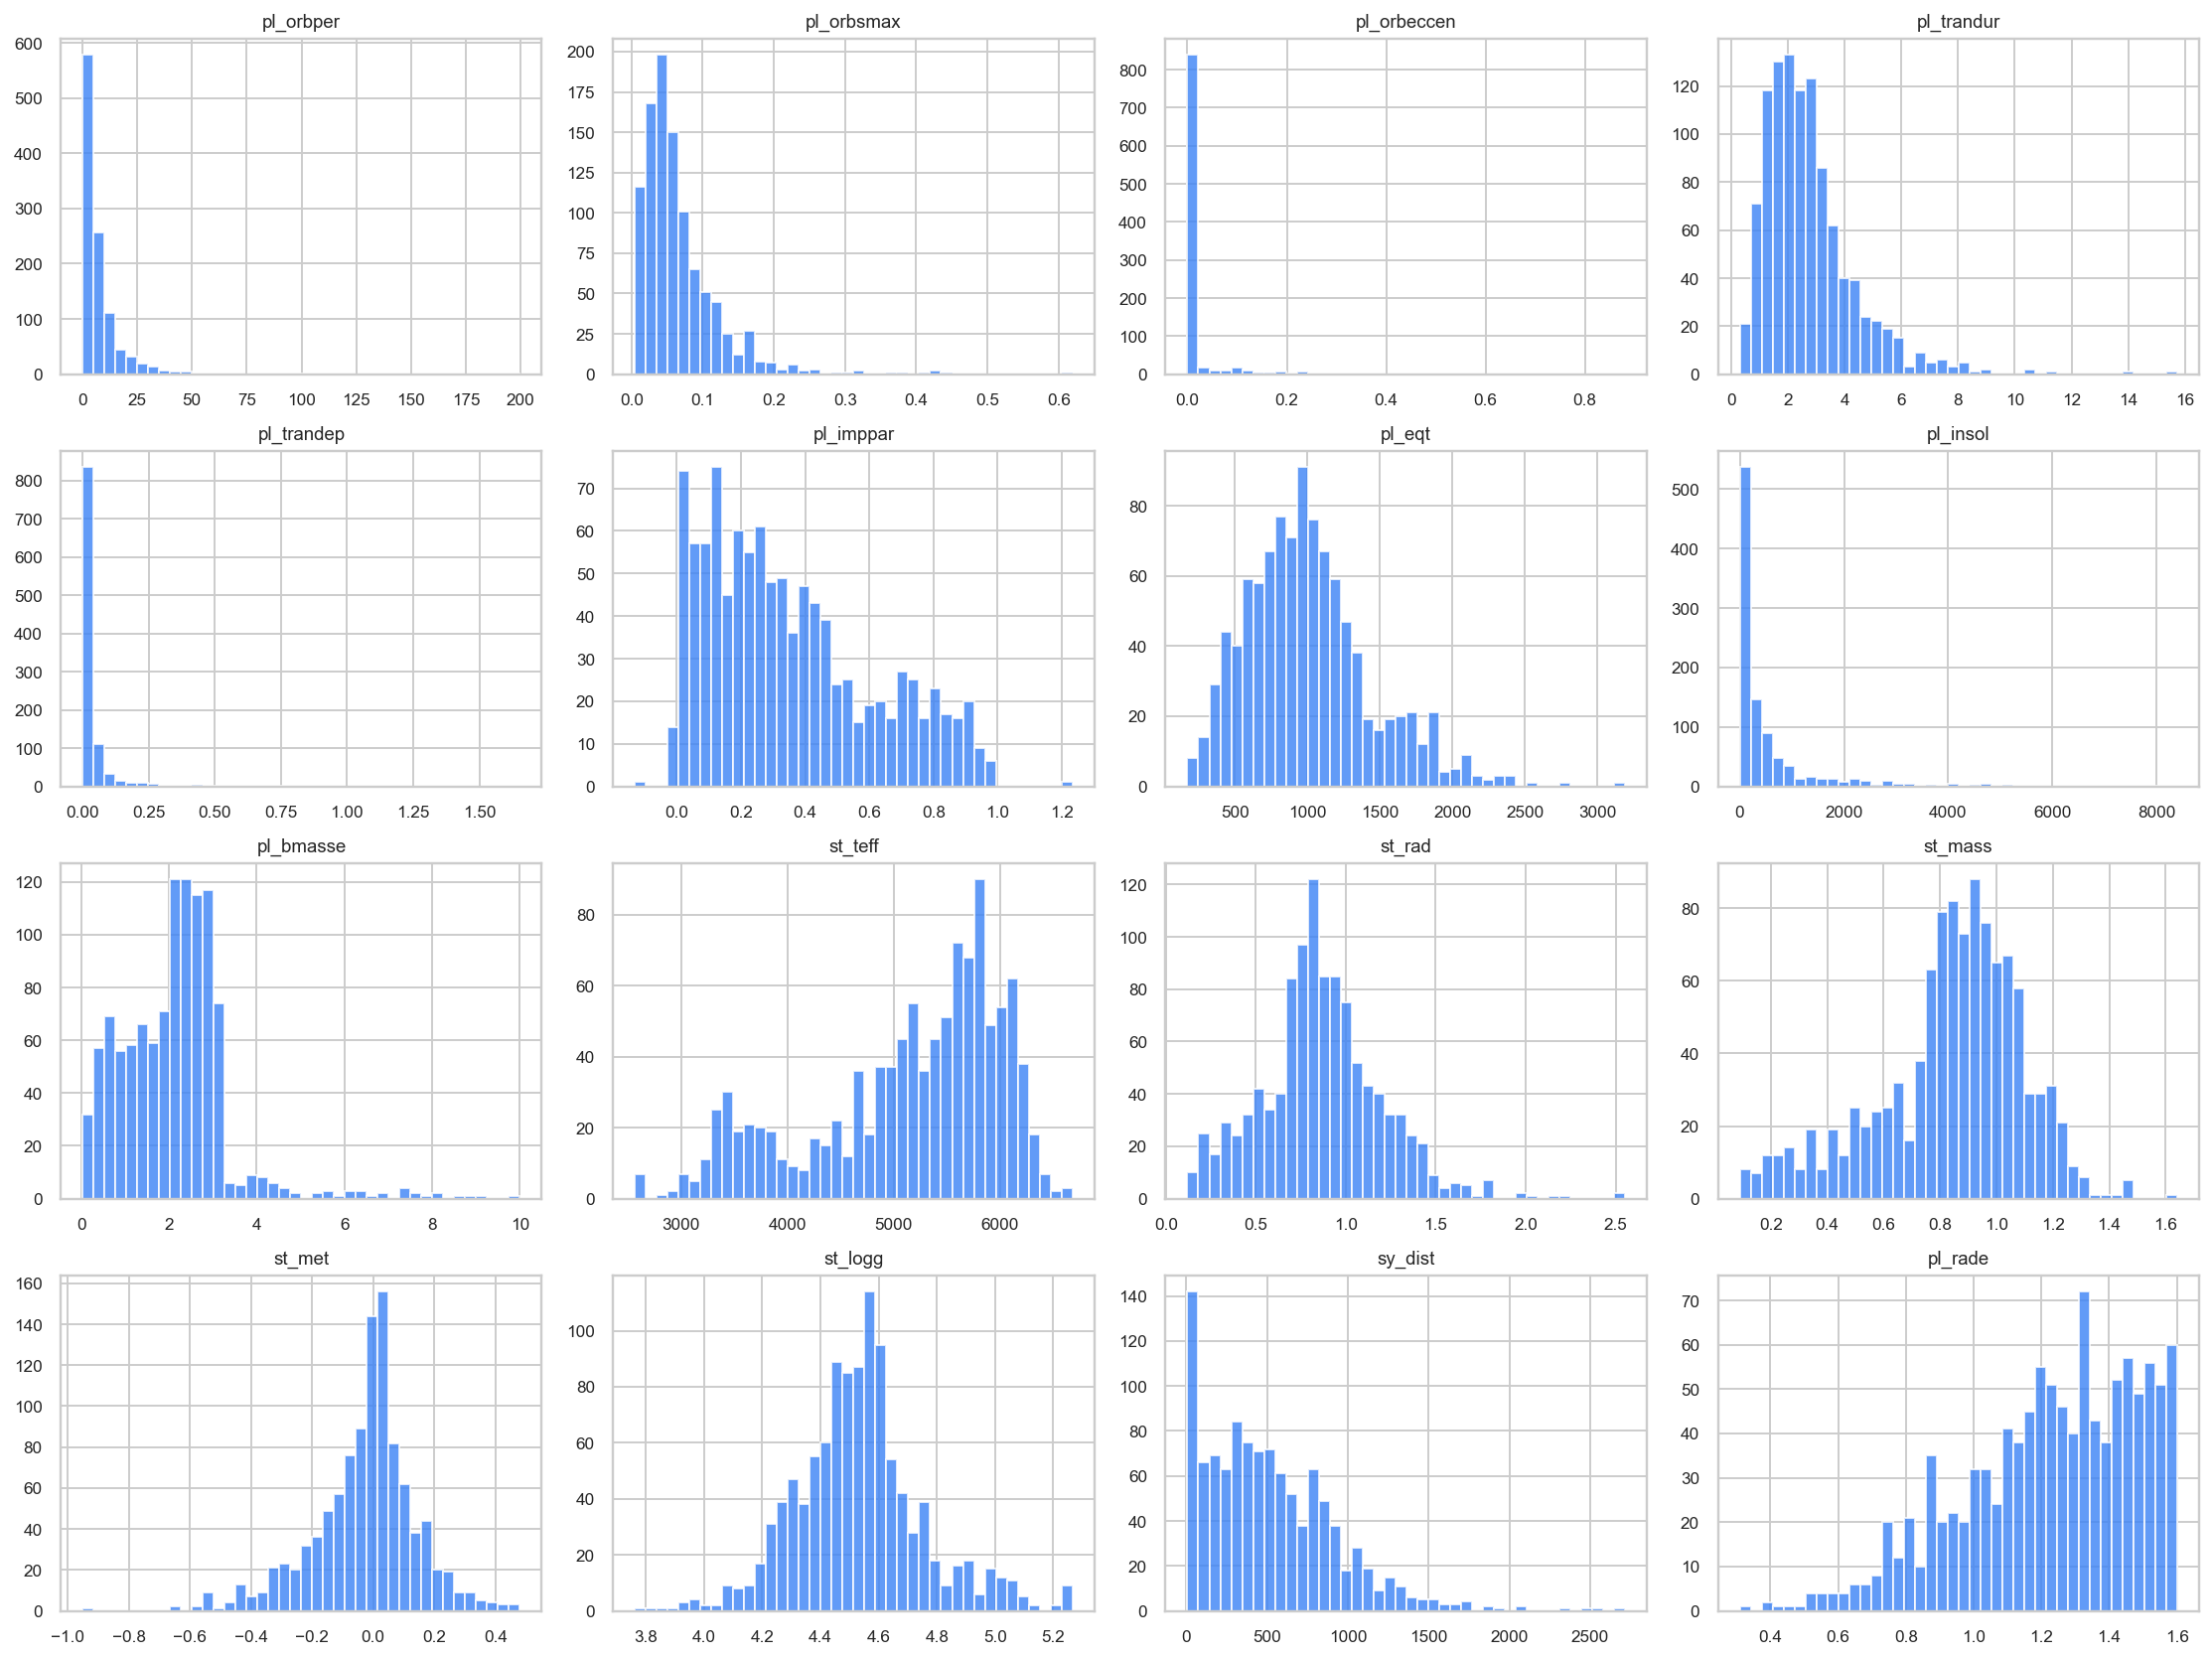
\includegraphics[width=\textwidth]{assets/part2/histograms.png}
    \caption{Histogram các biến số trước tiền xử lý. Nhiều biến có đuôi phải dài, đặc biệt là
    \texttt{pl\_orbper}, \texttt{pl\_insol}, \texttt{pl\_trandep} và \texttt{sy\_dist}.}
    \label{fig:part2_histograms}
\end{figure}

\begin{figure}[H]
    \centering
    
\includegraphics[width=0.95\textwidth]{assets/part2/correlation_heatmap.png}
    \caption{Ma trận tương quan Pearson. Các nhóm biến quỹ đạo/năng lượng như
    \texttt{pl\_orbper}, \texttt{pl\_orbsmax}, \texttt{pl\_eqt}, \texttt{pl\_insol} có tương quan
    đáng chú ý, nên cần kiểm tra đa cộng tuyến bằng VIF.}
    \label{fig:part2_corr}
\end{figure}

\begin{figure}[H]
    \centering
    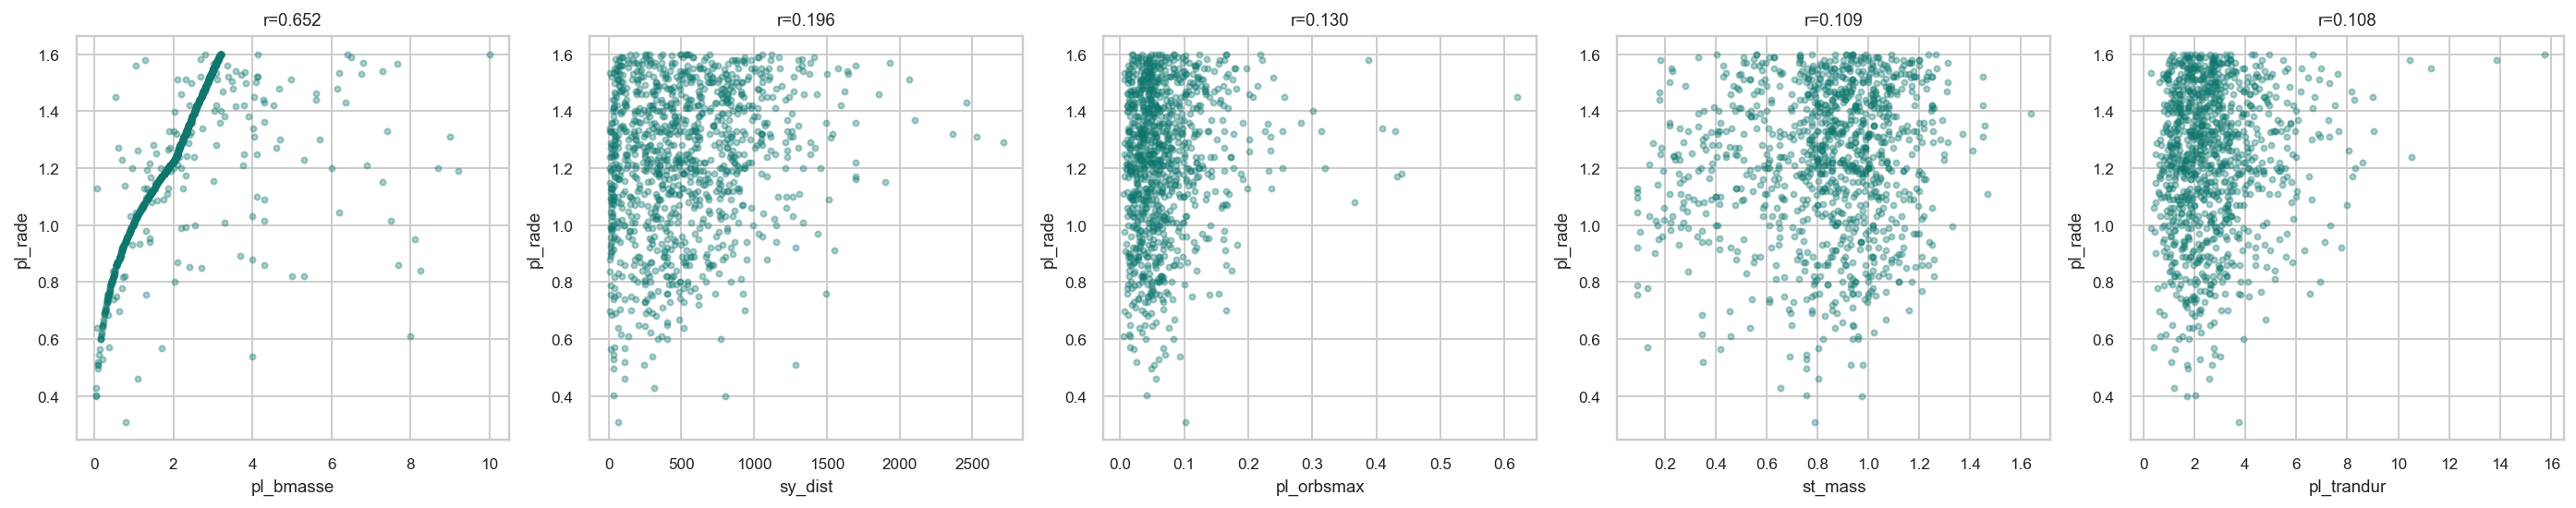
\includegraphics[width=\textwidth]{assets/part2/scatter_top5_target.png}
    \caption{Scatter plot giữa target \texttt{pl\_rade} và các biến có tương quan cao nhất.
    Quan hệ giữa target và predictors có xu hướng tuyến tính cục bộ nhưng vẫn còn nhiễu và ngoại lai.}
    \label{fig:part2_scatter}
\end{figure}

\subsubsection{Kiểm tra chất lượng dữ liệu}

Tương tự ví dụ tham khảo, nhóm kiểm tra bốn nhóm vấn đề: dữ liệu trùng lặp, dữ liệu khuyết, dữ liệu
nhiễu/ngoại lai và dữ liệu mâu thuẫn.

\paragraph{Dữ liệu trùng lặp.}
Trên 1084 mẫu sau domain restriction, số dòng trùng lặp bằng 0.

\begin{table}[H]
\centering
\caption{Kiểm tra duplicate sau domain restriction}
\label{tab:part2_duplicates}
\begin{tabular}{@{}lr@{}}
\hline
\textbf{Chỉ tiêu} & \textbf{Giá trị} \\
\hline
Số dòng kiểm tra & 1084 \\
Số dòng duplicate & 0 \\
\hline
\end{tabular}
\end{table}

\paragraph{Dữ liệu khuyết.}
Missing values xuất hiện ở nhiều nhóm biến khác nhau. Nếu xóa toàn bộ dòng chứa missing, dữ liệu sẽ
bị giảm đáng kể và dễ lệch mẫu; vì vậy pipeline dùng MICE ở bước tiền xử lý.

Lý do chọn MICE (\emph{Multiple Imputation by Chained Equations}) là dữ liệu ngoại hành tinh bị
khuyết theo nhiều nhóm phép đo khác nhau, trong khi các biến vật lý vẫn có quan hệ cấu trúc với
nhau. Ví dụ, bán trục lớn quỹ đạo, thông lượng bức xạ, nhiệt độ cân bằng, khối lượng hành tinh và
đặc trưng sao chủ không độc lập hoàn toàn. Nếu thay missing bằng trung bình/median đơn giản, mô
hình sẽ làm phẳng phương sai và bỏ qua quan hệ giữa các biến; nếu xóa dòng, tập dữ liệu còn lại dễ
thiên lệch về những hành tinh được quan sát đầy đủ hơn. MICE phù hợp hơn vì lần lượt xem từng cột
khuyết như một bài toán hồi quy có điều kiện trên các cột còn lại, nhờ đó giá trị điền vào giữ được
tương quan đa biến tốt hơn. Trong pipeline, MICE chỉ được fit trên train set rồi áp dụng sang test
set bằng các tham số đã học, nên bước điền khuyết không làm rò rỉ thông tin từ tập đánh giá.

\begin{table}[H]
\centering
\caption{Các cột có missing values nhiều nhất trước tiền xử lý}
\label{tab:part2_missing_eda}
\begin{tabular}{@{}lrrl@{}}
\hline
\textbf{Cột} & \textbf{Missing count} & \textbf{Missing (\%)} & \textbf{Kiểu dữ liệu} \\
\hline
\texttt{pl\_orbeccen} & 145 & 13.376 & float64 \\
\texttt{pl\_insol} & 103 & 9.502 & float64 \\
\texttt{pl\_orbsmax} & 86 & 7.934 & float64 \\
\texttt{pl\_eqt} & 79 & 7.288 & float64 \\
\texttt{pl\_trandep} & 51 & 4.705 & float64 \\
\texttt{pl\_imppar} & 44 & 4.059 & float64 \\
\texttt{st\_met} & 35 & 3.229 & float64 \\
\texttt{pl\_trandur} & 24 & 2.214 & float64 \\
\texttt{sy\_dist} & 6 & 0.554 & float64 \\
\hline
\end{tabular}
\end{table}

\paragraph{Dữ liệu nhiễu và ngoại lai.}
Một số biến có khoảng giá trị rất rộng, chẳng hạn \texttt{pl\_insol} có max 8385.9 trong khi median
chỉ 182.375. \texttt{pl\_trandep} cũng có skewness ban đầu 10.1802. Những giá trị cực trị này có
thể là quan sát thật trong thiên văn học, nên nhóm không xóa dòng mà dùng log-transform và
Winsorization để giảm ảnh hưởng đòn bẩy.

\paragraph{Dữ liệu mâu thuẫn.}
Các biến chính như chu kỳ quỹ đạo, khối lượng, bán kính, nhiệt độ sao và khoảng cách đều nằm trong
miền vật lý dương sau khi chọn mẫu. Biến \texttt{pl\_imppar} có min $-0.13$ và max $1.2325$, có thể
đến từ sai số fitting trong dữ liệu quan trắc transit. Nhóm không xem đây là conflict data để xóa
cứng; thay vào đó bước Winsorization sẽ giới hạn ảnh hưởng của các giá trị cực trị trên tập train.


